\chapter{Dataset Forensic Analysis and Integrity Audit}
\label{chap:dataset_forensics}

Before executing machine learning experiments, an independent empirical forensic audit was performed directly on the raw files (\texttt{Training.csv} and \texttt{Testing.csv}) from the Kaggle Disease Prediction repository~\cite{kaushil2020kaggle}.

\begin{table}[H]
\caption{Empirical Forensic Audit of the Kaggle Disease Dataset}
\label{tab:forensic_summary}
\centering
\begin{tabular}{lll}
\toprule
\textbf{Forensic Dimension} & \textbf{Published Claim} & \textbf{Empirical Ground Truth} \\
\midrule
Training Records & 4,920 & 4,920 records \\
Testing Records & 42 & 42 records \\
Symptom Features & 132 binary & 132 binary ($x_i \in \{0, 1\}$) \\
Artifact Columns & Not mentioned & 1 empty col (\texttt{Unnamed: 133}) \\
Disease Classes & \textbf{42 diseases} & \textbf{41 unique diseases} \\
Training Class Balance & Not specified & Perfectly balanced (120/class) \\
Unique Feature Vectors & Not specified & \textbf{304 unique vectors} \\
Exact Train Duplicates & Not specified & \textbf{4,616 records (93.82\%)} \\
Contradictory Vectors & Not specified & 0 contradictions \\
Train-Test Overlap & Independent test & \textbf{41 of 42 records (97.62\%)} \\
Mean Active Symptoms & Not specified & \textbf{7.45 $\pm$ 3.59} (Range: 3--17) \\
\bottomrule
\end{tabular}
\end{table}

\section{Forensic Finding 1: The 41 vs. 42 Disease Discrepancy}
\label{sec:forensic_finding1}
The Kaggle dataset documentation claims coverage of 42 distinct disease entities. However, programmatic inspection reveals exactly 41 unique labels in both \texttt{Training.csv} and \texttt{Testing.csv}. In the training set, each of the 41 classes has exactly 120 samples ($41 \times 120 = 4{,}920$). In the testing set, 40 diseases have exactly 1 sample, while one disease (\emph{Fungal infection}) has 2 samples ($40 \times 1 + 1 \times 2 = 42$). The published claim of ``42 diseases'' was evidently an error arising from conflating the 42 test records with the number of classes.

\section{Forensic Finding 2: Synthetic Redundancy and Duplication}
\label{sec:forensic_finding2}
As documented in Table~\ref{tab:forensic_summary}, while the training dataset contains 4,920 rows, it comprises only \textbf{304 unique symptom vectors}. Exactly 4,616 rows (93.82\%) are verbatim duplicate copies. As illustrated in \cref{fig:patterns_per_disease}, each disease is defined by only 5 to 10 unique symptom patterns replicated 12 to 24 times.

\begin{figure}[H]
\centering
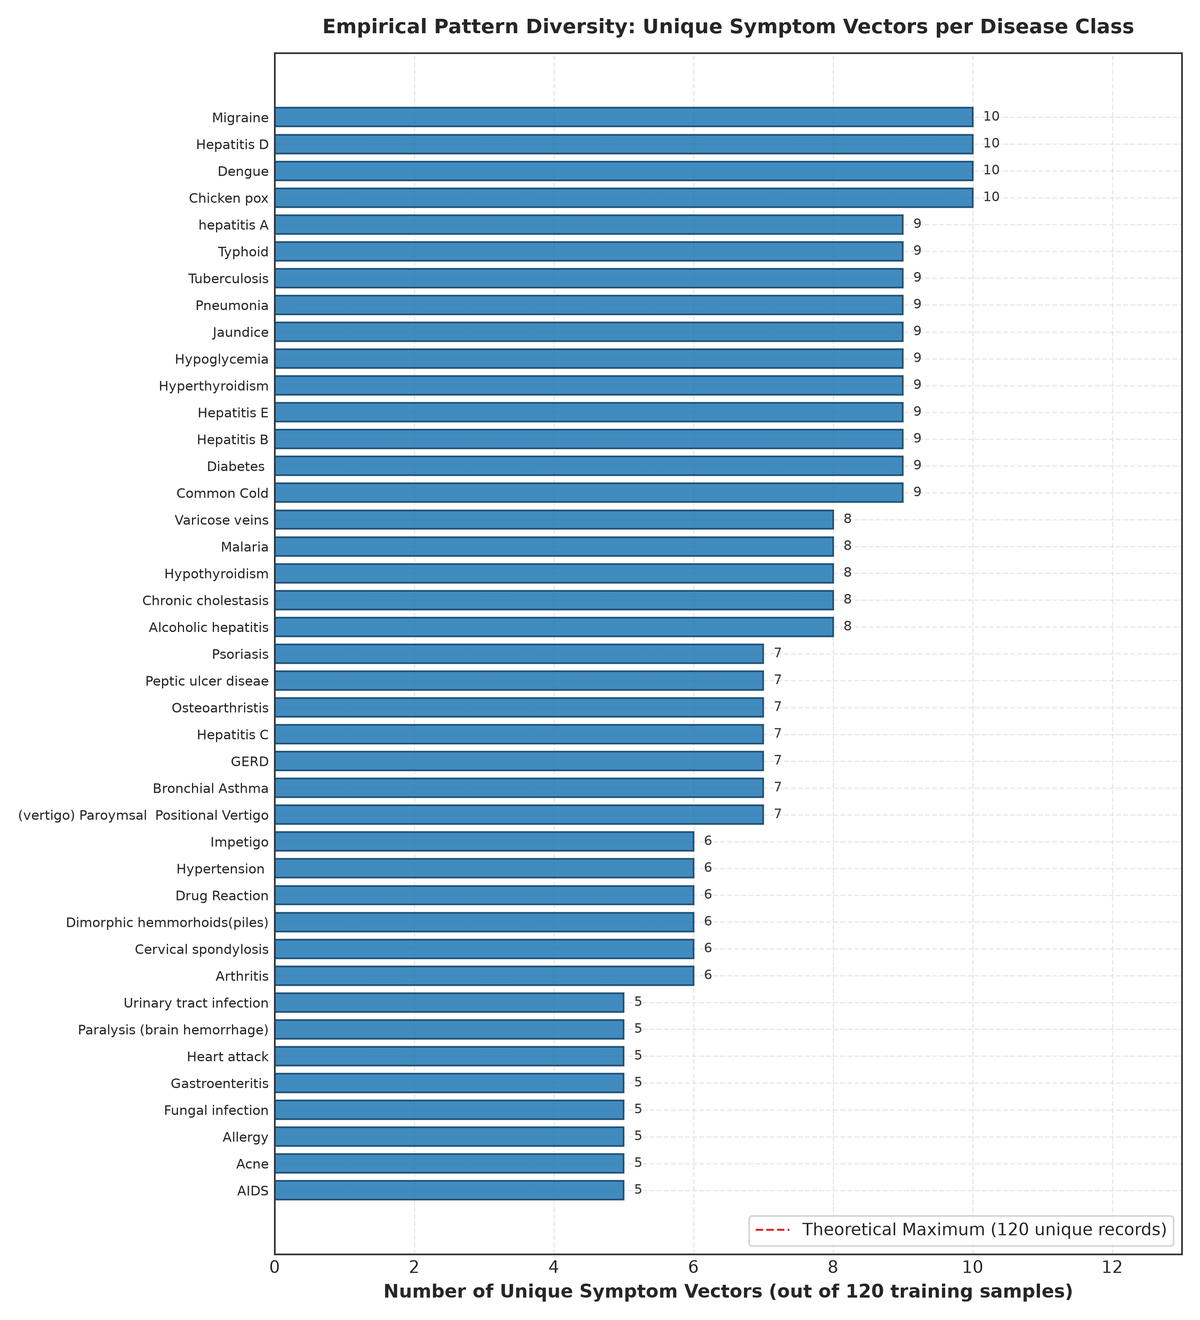
\includegraphics[width=0.9\textwidth]{fig1_unique_patterns_per_disease.png}
\caption{Empirical pattern diversity: Number of unique symptom vectors per disease class (out of 120 training records). Replicated synthetic vectors dominate the cohort.}
\label{fig:patterns_per_disease}
\end{figure}

\begin{figure}[H]
\centering
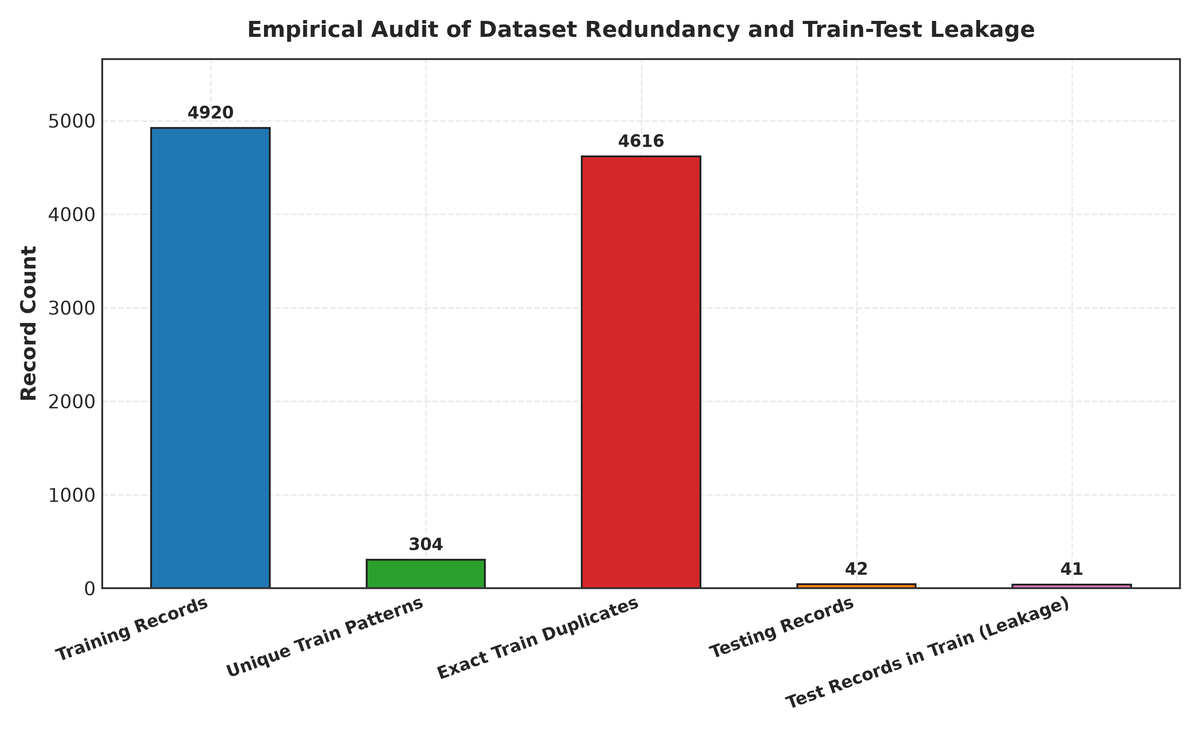
\includegraphics[width=0.9\textwidth]{fig4_redundancy_and_leakage_audit.png}
\caption{Empirical audit of dataset redundancy and train-test leakage. Out of 42 test records, 41 are exact duplicate copies of training records.}
\label{fig:leakage_audit}
\end{figure}

\section{Forensic Finding 3: Severe Train-Test Data Leakage}
\label{sec:forensic_finding3}
Crucially, set-theoretic intersection between the test and training sets confirms that \textbf{41 out of 42 testing records (97.62\%) are identical duplicates of training records} (\cref{fig:leakage_audit}). In the formal taxonomy of data leakage established by Kaufman et al.~\cite{kaufman2012leakage} and Kapoor and Narayanan~\cite{kapoor2023leakage}, this constitutes complete train-test contamination: evaluating models using the Kaggle test set does not measure generalizable predictive modeling, but rather verbatim vector retrieval from memorized training instances.
